

\tikzset{every picture/.style={line width=0.75pt}} %set default line width to 0.75pt        

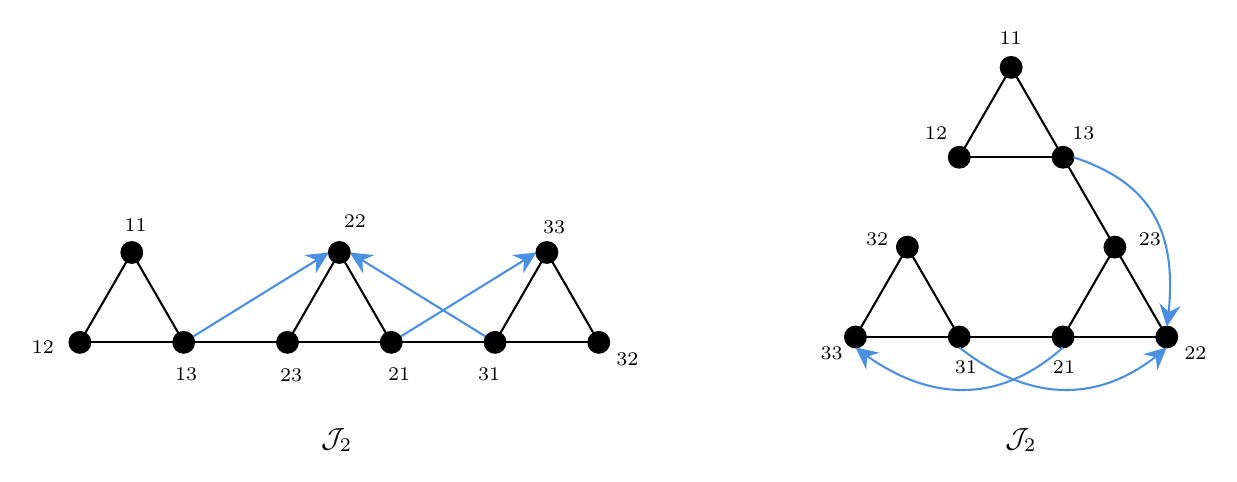
\begin{tikzpicture}[x=0.75pt,y=0.75pt,yscale=-1,xscale=1]
%uncomment if require: \path (0,548); %set diagram left start at 0, and has height of 548

%Straight Lines [id:da2456517091785999] 
\draw [color={rgb, 255:red, 74; green, 144; blue, 226 }  ,draw opacity=1 ]   (75.67,162.18) -- (143.12,120.46) ;
\draw [shift={(145.67,118.88)}, rotate = 148.26] [fill={rgb, 255:red, 74; green, 144; blue, 226 }  ,fill opacity=1 ][line width=0.08]  [draw opacity=0] (10.72,-5.15) -- (0,0) -- (10.72,5.15) -- (7.12,0) -- cycle    ;
%Straight Lines [id:da022114268321746122] 
\draw [color={rgb, 255:red, 74; green, 144; blue, 226 }  ,draw opacity=1 ]   (225.67,162.18) -- (158.22,120.46) ;
\draw [shift={(155.67,118.88)}, rotate = 31.74] [fill={rgb, 255:red, 74; green, 144; blue, 226 }  ,fill opacity=1 ][line width=0.08]  [draw opacity=0] (10.72,-5.15) -- (0,0) -- (10.72,5.15) -- (7.12,0) -- cycle    ;
%Straight Lines [id:da66595358457143] 
\draw [color={rgb, 255:red, 74; green, 144; blue, 226 }  ,draw opacity=1 ]   (175.67,162.18) -- (243.12,120.46) ;
\draw [shift={(245.67,118.88)}, rotate = 148.26] [fill={rgb, 255:red, 74; green, 144; blue, 226 }  ,fill opacity=1 ][line width=0.08]  [draw opacity=0] (10.72,-5.15) -- (0,0) -- (10.72,5.15) -- (7.12,0) -- cycle    ;
%Shape: Circle [id:dp9424970590435144] 
\draw  [fill={rgb, 255:red, 0; green, 0; blue, 0 }  ,fill opacity=1 ] (45.67,118.88) .. controls (45.67,116.12) and (47.91,113.88) .. (50.67,113.88) .. controls (53.43,113.88) and (55.67,116.12) .. (55.67,118.88) .. controls (55.67,121.64) and (53.43,123.88) .. (50.67,123.88) .. controls (47.91,123.88) and (45.67,121.64) .. (45.67,118.88) -- cycle ;
%Shape: Circle [id:dp6847867911902896] 
\draw  [fill={rgb, 255:red, 0; green, 0; blue, 0 }  ,fill opacity=1 ] (20.67,162.18) .. controls (20.67,159.42) and (22.91,157.18) .. (25.67,157.18) .. controls (28.43,157.18) and (30.67,159.42) .. (30.67,162.18) .. controls (30.67,164.95) and (28.43,167.18) .. (25.67,167.18) .. controls (22.91,167.18) and (20.67,164.95) .. (20.67,162.18) -- cycle ;
%Straight Lines [id:da8778413230089157] 
\draw [fill={rgb, 255:red, 208; green, 2; blue, 27 }  ,fill opacity=1 ]   (25.67,162.18) -- (75.67,162.18) ;
%Shape: Circle [id:dp17471639965887364] 
\draw  [fill={rgb, 255:red, 0; green, 0; blue, 0 }  ,fill opacity=1 ] (70.67,162.18) .. controls (70.67,159.42) and (72.91,157.18) .. (75.67,157.18) .. controls (78.43,157.18) and (80.67,159.42) .. (80.67,162.18) .. controls (80.67,164.95) and (78.43,167.18) .. (75.67,167.18) .. controls (72.91,167.18) and (70.67,164.95) .. (70.67,162.18) -- cycle ;
%Straight Lines [id:da18636404150658192] 
\draw [fill={rgb, 255:red, 208; green, 2; blue, 27 }  ,fill opacity=1 ]   (50.67,118.88) -- (25.67,162.18) ;
%Straight Lines [id:da8211638709625586] 
\draw [fill={rgb, 255:red, 208; green, 2; blue, 27 }  ,fill opacity=1 ]   (50.67,118.88) -- (75.67,162.18) ;
%Straight Lines [id:da6979444395661007] 
\draw    (75.67,162.18) -- (125.67,162.18) ;
%Shape: Circle [id:dp2498766628203688] 
\draw  [fill={rgb, 255:red, 0; green, 0; blue, 0 }  ,fill opacity=1 ] (120.67,162.18) .. controls (120.67,159.42) and (122.91,157.18) .. (125.67,157.18) .. controls (128.43,157.18) and (130.67,159.42) .. (130.67,162.18) .. controls (130.67,164.95) and (128.43,167.18) .. (125.67,167.18) .. controls (122.91,167.18) and (120.67,164.95) .. (120.67,162.18) -- cycle ;
%Straight Lines [id:da7632849580794818] 
\draw    (125.67,162.18) -- (175.67,162.18) ;
%Shape: Circle [id:dp23013565246057377] 
\draw  [fill={rgb, 255:red, 0; green, 0; blue, 0 }  ,fill opacity=1 ] (170.67,162.18) .. controls (170.67,159.42) and (172.91,157.18) .. (175.67,157.18) .. controls (178.43,157.18) and (180.67,159.42) .. (180.67,162.18) .. controls (180.67,164.95) and (178.43,167.18) .. (175.67,167.18) .. controls (172.91,167.18) and (170.67,164.95) .. (170.67,162.18) -- cycle ;
%Straight Lines [id:da25360390235593866] 
\draw    (175.67,162.18) -- (225.67,162.18) ;
%Straight Lines [id:da4057846208592779] 
\draw    (225.67,162.18) -- (275.67,162.18) ;
%Shape: Circle [id:dp20540786701918234] 
\draw  [fill={rgb, 255:red, 0; green, 0; blue, 0 }  ,fill opacity=1 ] (220.67,162.18) .. controls (220.67,159.42) and (222.91,157.18) .. (225.67,157.18) .. controls (228.43,157.18) and (230.67,159.42) .. (230.67,162.18) .. controls (230.67,164.95) and (228.43,167.18) .. (225.67,167.18) .. controls (222.91,167.18) and (220.67,164.95) .. (220.67,162.18) -- cycle ;
%Shape: Circle [id:dp6839097721394887] 
\draw  [fill={rgb, 255:red, 0; green, 0; blue, 0 }  ,fill opacity=1 ] (145.67,118.88) .. controls (145.67,116.12) and (147.91,113.88) .. (150.67,113.88) .. controls (153.43,113.88) and (155.67,116.12) .. (155.67,118.88) .. controls (155.67,121.64) and (153.43,123.88) .. (150.67,123.88) .. controls (147.91,123.88) and (145.67,121.64) .. (145.67,118.88) -- cycle ;
%Straight Lines [id:da12323183009990557] 
\draw [fill={rgb, 255:red, 208; green, 2; blue, 27 }  ,fill opacity=1 ]   (150.67,118.88) -- (125.67,162.18) ;
%Straight Lines [id:da7588294087224081] 
\draw [fill={rgb, 255:red, 208; green, 2; blue, 27 }  ,fill opacity=1 ]   (150.67,118.88) -- (175.67,162.18) ;
%Shape: Circle [id:dp9571324776779264] 
\draw  [fill={rgb, 255:red, 0; green, 0; blue, 0 }  ,fill opacity=1 ] (270.67,162.18) .. controls (270.67,159.42) and (272.91,157.18) .. (275.67,157.18) .. controls (278.43,157.18) and (280.67,159.42) .. (280.67,162.18) .. controls (280.67,164.95) and (278.43,167.18) .. (275.67,167.18) .. controls (272.91,167.18) and (270.67,164.95) .. (270.67,162.18) -- cycle ;
%Shape: Circle [id:dp4379827116422321] 
\draw  [fill={rgb, 255:red, 0; green, 0; blue, 0 }  ,fill opacity=1 ] (245.67,118.88) .. controls (245.67,116.12) and (247.91,113.88) .. (250.67,113.88) .. controls (253.43,113.88) and (255.67,116.12) .. (255.67,118.88) .. controls (255.67,121.64) and (253.43,123.88) .. (250.67,123.88) .. controls (247.91,123.88) and (245.67,121.64) .. (245.67,118.88) -- cycle ;
%Straight Lines [id:da1136043779778182] 
\draw [fill={rgb, 255:red, 208; green, 2; blue, 27 }  ,fill opacity=1 ]   (250.67,118.88) -- (225.67,162.18) ;
%Straight Lines [id:da8583414213334941] 
\draw [fill={rgb, 255:red, 208; green, 2; blue, 27 }  ,fill opacity=1 ]   (250.67,118.88) -- (275.67,162.18) ;

%Straight Lines [id:da6246212882143305] 
\draw [fill={rgb, 255:red, 208; green, 2; blue, 27 }  ,fill opacity=1 ]   (449.33,73) -- (499.33,73) ;
%Straight Lines [id:da3527263833875742] 
\draw [fill={rgb, 255:red, 208; green, 2; blue, 27 }  ,fill opacity=1 ]   (474.33,29.7) -- (499.33,73) ;
%Straight Lines [id:da6692966739575246] 
\draw [fill={rgb, 255:red, 208; green, 2; blue, 27 }  ,fill opacity=1 ]   (474.33,29.7) -- (449.33,73) ;
%Shape: Circle [id:dp13029704254607122] 
\draw  [fill={rgb, 255:red, 0; green, 0; blue, 0 }  ,fill opacity=1 ] (469.33,29.7) .. controls (469.33,26.94) and (471.57,24.7) .. (474.33,24.7) .. controls (477.09,24.7) and (479.33,26.94) .. (479.33,29.7) .. controls (479.33,32.46) and (477.09,34.7) .. (474.33,34.7) .. controls (471.57,34.7) and (469.33,32.46) .. (469.33,29.7) -- cycle ;
%Shape: Circle [id:dp2929238979439357] 
\draw  [fill={rgb, 255:red, 0; green, 0; blue, 0 }  ,fill opacity=1 ] (444.33,73) .. controls (444.33,70.24) and (446.57,68) .. (449.33,68) .. controls (452.09,68) and (454.33,70.24) .. (454.33,73) .. controls (454.33,75.76) and (452.09,78) .. (449.33,78) .. controls (446.57,78) and (444.33,75.76) .. (444.33,73) -- cycle ;
%Shape: Circle [id:dp1932098096298014] 
\draw  [fill={rgb, 255:red, 0; green, 0; blue, 0 }  ,fill opacity=1 ] (494.33,73) .. controls (494.33,70.24) and (496.57,68) .. (499.33,68) .. controls (502.09,68) and (504.33,70.24) .. (504.33,73) .. controls (504.33,75.76) and (502.09,78) .. (499.33,78) .. controls (496.57,78) and (494.33,75.76) .. (494.33,73) -- cycle ;
%Straight Lines [id:da8055342090019448] 
\draw [fill={rgb, 255:red, 208; green, 2; blue, 27 }  ,fill opacity=1 ]   (424.33,116.3) -- (399.33,159.6) ;
%Straight Lines [id:da8415811249013536] 
\draw    (499.33,73) -- (524.33,116.3) ;
%Straight Lines [id:da4896953572060836] 
\draw [fill={rgb, 255:red, 208; green, 2; blue, 27 }  ,fill opacity=1 ]   (524.33,116.3) -- (549.33,159.6) ;
%Straight Lines [id:da12654072525376492] 
\draw [fill={rgb, 255:red, 208; green, 2; blue, 27 }  ,fill opacity=1 ]   (524.33,116.3) -- (499.33,159.6) ;
%Straight Lines [id:da5313555995209134] 
\draw [fill={rgb, 255:red, 208; green, 2; blue, 27 }  ,fill opacity=1 ]   (424.33,116.3) -- (449.33,159.6) ;
%Straight Lines [id:da805969047450577] 
\draw [fill={rgb, 255:red, 208; green, 2; blue, 27 }  ,fill opacity=1 ]   (399.33,159.6) -- (449.33,159.6) ;
%Straight Lines [id:da0884017129215724] 
\draw [fill={rgb, 255:red, 208; green, 2; blue, 27 }  ,fill opacity=1 ]   (499.33,159.6) -- (549.33,159.6) ;
%Straight Lines [id:da3104775657586403] 
\draw    (449.33,159.6) -- (499.33,159.6) ;
%Shape: Circle [id:dp27232767475177355] 
\draw  [fill={rgb, 255:red, 0; green, 0; blue, 0 }  ,fill opacity=1 ] (544.33,159.6) .. controls (544.33,156.84) and (546.57,154.6) .. (549.33,154.6) .. controls (552.09,154.6) and (554.33,156.84) .. (554.33,159.6) .. controls (554.33,162.36) and (552.09,164.6) .. (549.33,164.6) .. controls (546.57,164.6) and (544.33,162.36) .. (544.33,159.6) -- cycle ;
%Shape: Circle [id:dp3341291394413648] 
\draw  [fill={rgb, 255:red, 0; green, 0; blue, 0 }  ,fill opacity=1 ] (494.33,159.6) .. controls (494.33,156.84) and (496.57,154.6) .. (499.33,154.6) .. controls (502.09,154.6) and (504.33,156.84) .. (504.33,159.6) .. controls (504.33,162.36) and (502.09,164.6) .. (499.33,164.6) .. controls (496.57,164.6) and (494.33,162.36) .. (494.33,159.6) -- cycle ;
%Shape: Circle [id:dp8277296739836901] 
\draw  [fill={rgb, 255:red, 0; green, 0; blue, 0 }  ,fill opacity=1 ] (519.33,116.3) .. controls (519.33,113.54) and (521.57,111.3) .. (524.33,111.3) .. controls (527.09,111.3) and (529.33,113.54) .. (529.33,116.3) .. controls (529.33,119.06) and (527.09,121.3) .. (524.33,121.3) .. controls (521.57,121.3) and (519.33,119.06) .. (519.33,116.3) -- cycle ;
%Shape: Circle [id:dp26171943798388275] 
\draw  [fill={rgb, 255:red, 0; green, 0; blue, 0 }  ,fill opacity=1 ] (444.33,159.6) .. controls (444.33,156.84) and (446.57,154.6) .. (449.33,154.6) .. controls (452.09,154.6) and (454.33,156.84) .. (454.33,159.6) .. controls (454.33,162.36) and (452.09,164.6) .. (449.33,164.6) .. controls (446.57,164.6) and (444.33,162.36) .. (444.33,159.6) -- cycle ;
%Shape: Circle [id:dp570427538306592] 
\draw  [fill={rgb, 255:red, 0; green, 0; blue, 0 }  ,fill opacity=1 ] (394.33,159.6) .. controls (394.33,156.84) and (396.57,154.6) .. (399.33,154.6) .. controls (402.09,154.6) and (404.33,156.84) .. (404.33,159.6) .. controls (404.33,162.36) and (402.09,164.6) .. (399.33,164.6) .. controls (396.57,164.6) and (394.33,162.36) .. (394.33,159.6) -- cycle ;
%Shape: Circle [id:dp021872500246036708] 
\draw  [fill={rgb, 255:red, 0; green, 0; blue, 0 }  ,fill opacity=1 ] (419.33,116.3) .. controls (419.33,113.54) and (421.57,111.3) .. (424.33,111.3) .. controls (427.09,111.3) and (429.33,113.54) .. (429.33,116.3) .. controls (429.33,119.06) and (427.09,121.3) .. (424.33,121.3) .. controls (421.57,121.3) and (419.33,119.06) .. (419.33,116.3) -- cycle ;
%Curve Lines [id:da4398310068180369] 
\draw [color={rgb, 255:red, 74; green, 144; blue, 226 }  ,draw opacity=1 ]   (504.33,73) .. controls (541.84,85.26) and (555.29,109.08) .. (549.7,151.95) ;
\draw [shift={(549.33,154.6)}, rotate = 278.3] [fill={rgb, 255:red, 74; green, 144; blue, 226 }  ,fill opacity=1 ][line width=0.08]  [draw opacity=0] (10.72,-5.15) -- (0,0) -- (10.72,5.15) -- (7.12,0) -- cycle    ;
%Curve Lines [id:da8489853946203825] 
\draw [color={rgb, 255:red, 74; green, 144; blue, 226 }  ,draw opacity=1 ]   (499.33,164.6) .. controls (469.96,190.96) and (436.05,192.45) .. (401.45,166.24) ;
\draw [shift={(399.33,164.6)}, rotate = 38.3] [fill={rgb, 255:red, 74; green, 144; blue, 226 }  ,fill opacity=1 ][line width=0.08]  [draw opacity=0] (10.72,-5.15) -- (0,0) -- (10.72,5.15) -- (7.12,0) -- cycle    ;
%Curve Lines [id:da8681887944950593] 
\draw [color={rgb, 255:red, 74; green, 144; blue, 226 }  ,draw opacity=1 ]   (546.62,166.95) .. controls (517.28,191.53) and (483.6,191.67) .. (449.33,164.6) ;
\draw [shift={(549.33,164.6)}, rotate = 138.1] [fill={rgb, 255:red, 74; green, 144; blue, 226 }  ,fill opacity=1 ][line width=0.08]  [draw opacity=0] (10.72,-5.15) -- (0,0) -- (10.72,5.15) -- (7.12,0) -- cycle    ;


% Text Node
\draw (470,202.4) node [anchor=north west][inner sep=0.75pt]    {$\mathcal{J}_{2}$};
% Text Node
\draw (1,160.22) node [anchor=north west][inner sep=0.75pt]  [font=\scriptsize]  {$12$};
% Text Node
\draw (120.67,173.55) node [anchor=north west][inner sep=0.75pt]  [font=\scriptsize]  {$23$};
% Text Node
\draw (45.67,101.22) node [anchor=north west][inner sep=0.75pt]  [font=\scriptsize]  {$11$};
% Text Node
\draw (70,172.89) node [anchor=north west][inner sep=0.75pt]  [font=\scriptsize]  {$13$};
% Text Node
\draw (151.33,99.55) node [anchor=north west][inner sep=0.75pt]  [font=\scriptsize]  {$22$};
% Text Node
\draw (172.67,172.82) node [anchor=north west][inner sep=0.75pt]  [font=\scriptsize]  {$21$};
% Text Node
\draw (216,172.82) node [anchor=north west][inner sep=0.75pt]  [font=\scriptsize]  {$31$};
% Text Node
\draw (282.67,165.58) node [anchor=north west][inner sep=0.75pt]  [font=\scriptsize]  {$32$};
% Text Node
\draw (247.33,102.22) node [anchor=north west][inner sep=0.75pt]  [font=\scriptsize]  {$33$};
% Text Node
\draw (467.33,11.07) node [anchor=north west][inner sep=0.75pt]  [font=\scriptsize]  {$11$};
% Text Node
\draw (556.33,163.07) node [anchor=north west][inner sep=0.75pt]  [font=\scriptsize]  {$22$};
% Text Node
\draw (381,163.07) node [anchor=north west][inner sep=0.75pt]  [font=\scriptsize]  {$33$};
% Text Node
\draw (502.33,57.07) node [anchor=north west][inner sep=0.75pt]  [font=\scriptsize]  {$13$};
% Text Node
\draw (431.33,57.07) node [anchor=north west][inner sep=0.75pt]  [font=\scriptsize]  {$12$};
% Text Node
\draw (493,169.67) node [anchor=north west][inner sep=0.75pt]  [font=\scriptsize]  {$21$};
% Text Node
\draw (534.33,108.07) node [anchor=north west][inner sep=0.75pt]  [font=\scriptsize]  {$23$};
% Text Node
\draw (445.67,169.67) node [anchor=north west][inner sep=0.75pt]  [font=\scriptsize]  {$31$};
% Text Node
\draw (403,108.07) node [anchor=north west][inner sep=0.75pt]  [font=\scriptsize]  {$32$};
% Text Node
\draw (140.33,202.4) node [anchor=north west][inner sep=0.75pt]    {$\mathcal{J}_{2}$};


\end{tikzpicture}